\chapter{The Final Solution}
\label{chp:5:FinaSolu}
In this chapter, a final design of a mass communication system, named Myriad, will be introduced. Firstly, the improvements on the requirements will be compared to the ones defined for the prototype from previous chapter. Later, the actual product's features, and its architecture will be discussed.

\section{The Improved Requirements}
\label{sec:5.1:ImprRequ}

Having seen the prototype in action made us to review the requirements, and bring the ones. Some of those requirements are shaped according to the feedbacks that we got at the Stanford \ac{HCI} group, as well as the organizations who do mass email communication on weekly basis to reach their community. Following sections will discussed those new features on the final product. 

\subsection{Assistant Support}
\label{subsec:5.1.1:AssiSupp}
As it it discussed in section \ref{subsec:4.1.1:Cust}, the standard that we want to achieve within a mass email communication is the most adequately personalized emails according to recipients with minimum effort on a researcher's side. The initial idea and the prototype brought several features as discussed in chapter \ref{chp:4:InitIdeaProt} for this purpose. However, if you consider the gold standard in the figure \ref{fig:ChartEffortCustom} we would like to achieve, the prototype still leaves effort on a researcher to accomplished a successful mass email campaign.
\vspace{1cm}

In order to minimize the efforts on the researcher's side, the additional assistants' involvement was considered. Therefore, a primary researcher will be able to share the tasks with permitted assistants. These tasks may be extracting information from the incoming answers or even writing replies to those answers. Hence, the primary researcher will only need to interact with the flow of a mass email campaign when there is situation where it requires primary researcher attention. However, the system still needs to provide the necessary features that we will see in the next sections to support the work flow in a mass email campaign, hence assistants will only need to interact with this work flow to let the continuation of the email campaign by providing answers with the email templates, and extract information as \ac{KVP}s.

\subsection{Dynamic Variables and \ac{KVP}s}
\label{subsec:5.1.2:DynmVariKVPs}
We introduced dynamic variables at the initial prototype, however it was only limited at the salutation of the email. Since it allows the personalization of emails easier, and email marketing applications also supports this feature in the same purpose in section \ref{subsec:3.3.3:EmaiMarktAppl}, the final product will also include this feature. As a result, application users can create \ac{KVP}s and use those keys in the content of the email message to be replaced dynamically by its value according to the recipients. Therefore, the extracted information from the emails will not just help us to gather information in an organized, but also use them to personalize the emails
\vspace{1cm}

As a result, instead of keeping the \ac{KVP}s in the system according to the responds, system should keep them according to the recipients itself. This is where the \ac{KVP}-idea differs from the prototype as well. So, we have now profiles of contacts for a campaign having all \ac{KVP}s of a recipients visible during the whole state of the conversation, not just at one message of the recipient. However, system should offer an option to hide individual \ac{KVP}s to avoid cluttering on the view, and keep the \ac{KVP} list with the ones that are actively used.

\vspace{1cm}
Importing the \ac{KVP}s should be done in several ways. One option is that system should be able to synchronize with an online spreadsheet, e.g. Google Spreadsheet, to get the \ac{KVP}s at the beginning of a campaign. This is a convenient way for the researchers since they are already familiar with spreadsheet environment. Other options should be a campaign-wide view and a contact specific view in the system. Also, system should allow to edit both keys and values in a campaign.

\subsection{Importing and Exporting Contacts and Their Information}
\label{subsec:5.1.3:ImpoExpoContInfo}
In the prototype, application user had to enter the basic information of the recipients such as first name, last name, and email address into the system manually. However, we realized while they were doing this, they use a spreadsheet and copy the contact information from there. This was also the case for their regular email client that they used for email campaigns. The applications that was investigated in section \ref{sec:3.3:Resul} had an option to import from spreadsheet to ease the process. Therefore, the system should offer an option to import contacts from the spreadsheet environment.
\vspace{1cm}

However, importing should not be limited only the basic information of the recipients. Since we already mentioned about importing \ac{KVP}s from spreadsheet in the previous section, system should detect and import the contact information and \ac{KVP}s related to that contact if it is available from a provided spreadsheet. 
\vspace{1cm}

System should provide a bi-directional synchronization, not just importing data from the spreadsheet. Therefore, system should provide an option to export contact information and their created \ac{KVP}s from the system to the spreadsheet. This will also gives a reporting functionality to the application users, where they can see all the contacts, and their extracted information from a campaign in one view.

\subsection{Interoperability with Other Email Clients}
\label{subsec:5.1.4:InteEmaiClie}
Even though we provide a new system for the users to conduct their mass email communication, there might be some cases where a mass email communication initiated in the user's regular email client, and the system is not aware of that campaign since it was not created with it. Application should provide an option to import those emails messages created with another email client in to the system by recognizing those annotated messages by the user.
\vspace{1cm}

Enabling the system to import email conversations from other email clients reduce the dependency on the application, and while a researcher continue to use their own email client, assigned assistants can take care of those imported emails by the researcher. We saw such a import feature in \ac{CRM} applications in section \ref{subsec:3.3.1:CRMAppl} as well, where a user is able to forward an email into the \ac{CRM} application, and system takes care of assigning the imported email to the corresponding recipient entry in the system.

\subsection{Automated Decision-Making and Notifications}
\label{subsec:5.1.5:AutoDeciMakiNoti}
Even though the involvement of assistants make the initial researcher's life easier, the system still needs to provide an automated approach to answer the emails whose status is clear in the flow of a mass email communication. Therefore, a rule based decision-making mechanism should be used, where users sets the values of the keys of \ac{KVP}s, and it triggers the action of sending an email to a respondent.
\vspace{1cm}

Since the application's only purpose is the managing mass email communication and each campaign results great amount of messages in the inbox, the system should provide notifications regarding what should be done next for each recipients. Labels added to the email conversation should state whose turn is next in the communication. For instance, by proving a label saying "You need to reply" to the application user, the state of the communication waits an action from a researcher or an assistant. In the same way the unread conversations and the conversation waiting an answer from the respondents should be also annotated in the similar fashion. System should also provide email notification to the assistants' email addresses to notify them there is an action waiting to be taken care of.

\section{Final System}
\label{sec:5.2:FinaSyst}
In this section, we will see that how the revised and improved requirements from section \ref{sec:5.1:ImprRequ} reflected to the final product, named "Myriad".

\subsection{Log-In and Campaigns Overview}
\label{subsec:5.2.1:CampOver}

As it was the same case for the prototype in section \ref{subsec:4.2.2:ProtSyst}, Myriad also requires a Gmail account to work with. The reason behind this is not just the popularity of the Gmail, but also that Stanford University uses Google Apps by default at university wide. Therefore, each member of the university has a Google account to use with Myriad. This also provides flexibility to use Myriad, because there is no registration form or sign in screen. All the requested Google's permissions from a Myriad's user and their descriptions can be found in appendix \ref{app:GoogPerm}.
\vspace{1cm}

After user sign in to the system, the first screen that they will see is the campaigns overview screen, in where all the created campaigns including the ones that are shared with the user (as a assistant) are shown as in the figure \ref{fig:CampaignsOverviewScreen}. It has a simple and a clean \ac{UI}, deferring from regular email clients to emphasize its focus on mass email communication.

\begin{figure}[htbp]
	\centering
	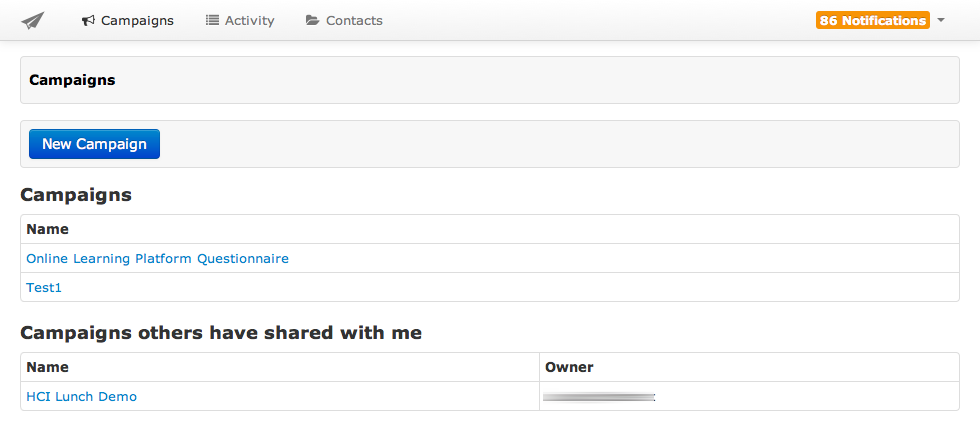
\includegraphics[width=1.00\textwidth]{imgs/CampaignsOverviewScreen.png}
	\caption[Myriad's Campaigns Overview Screen]{Myriad's Campaigns Overview Screen}
	\label{fig:CampaignsOverviewScreen}
\end{figure}

\subsection{Synchronization with Other Sytems}
\label{subsec:5.2.2:SyncOtheSyst}

Myriad is able to get the contacts' information and their \ac{KVP}s from Google Spreadsheet. This is a convenient way to import contacts into the system since many people already keeps their information in a spreadsheet environment as we discussed in section \ref{subsec:5.1.3:ImpoExpoContInfo}. Therefore, Myriad offers a bi-directional syncing from and to the spreadsheet defined at the creation of a campaign. Besides, Myriad also offers an option to enter recipients first name, last name, and email address into the system directly.
\vspace{1cm}

The corresponding columns in the spreadsheet start with "first name", "last name", and "email address" as in the figure \ref{fig:GoogleSpreadsheet}. The rest of the columns will be acted as a \ac{KVP}, and imported into the system as well.

\begin{figure}[htbp]
	\centering
	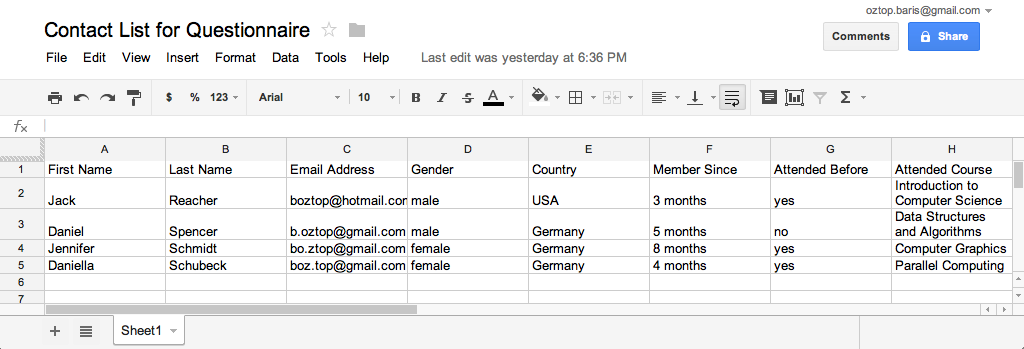
\includegraphics[width=1.00\textwidth]{imgs/GoogleSpreadsheet.png}
	\caption[A Google Spreadsheet to Import into Myriad]{A Google Spreadsheet to Import into Myriad}
	\label{fig:GoogleSpreadsheet}
\end{figure}

As it was discussed in section \ref{subsec:5.1.4:InteEmaiClie}, importing existing email conversations as campaigns into the system is an important feature, since researchers may initiate conversations in their regular email client, and later on to make them more manageable, they can import them into Myriad. Myriad leverages Gmail's labeling feature which is equivalent to the \ac{IMAP} protocol's folders for this purpose \citep{GoogleInc.2013}. Myriad creates a Gmail label in the user's account, and the only thing that user needs to do is the enable label syncing feature at the create campaign screen. Next, there will appear a label with the campaign name, and group under the root label of "myriad" in Gmail's inbox as in the figure \ref{fig:GmailLabels}. Hence, researcher will able to imports email messages, which were not considered to belong to a campaign for some reason, into Myriad.

\clearpage

\begin{figure}[htbp]
	\centering
	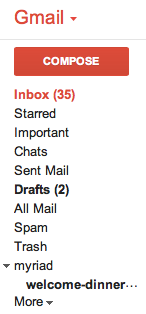
\includegraphics[scale=0.60]{imgs/GmailLabels.png}
	\caption[Gmail's Labels and the Myriad's Campaigns Under the Myriad Label]{Gmail's Labels and the Myriad's Campaigns Under the Myriad Label}
	\label{fig:GmailLabels}
\end{figure}

\subsection{Creating an Email Campaign}
\label{subsec:5.2.3:CreaEmaiCamp}

The campaign creation screen (see figure \ref{fig:CreateCampaign}) has input fields for a campaign name and Google Spreadsheet's URL to synchronize with. Other two checkboxes for the spreadsheet are to manage the frequency of synchronization and disabling the warning in case of erroneous data in the spreadsheet such as an empty email address field for a contact. The option for importing emails from Gmail's inbox is also in this screen under label synching.

\begin{figure}[htbp]
	\centering
	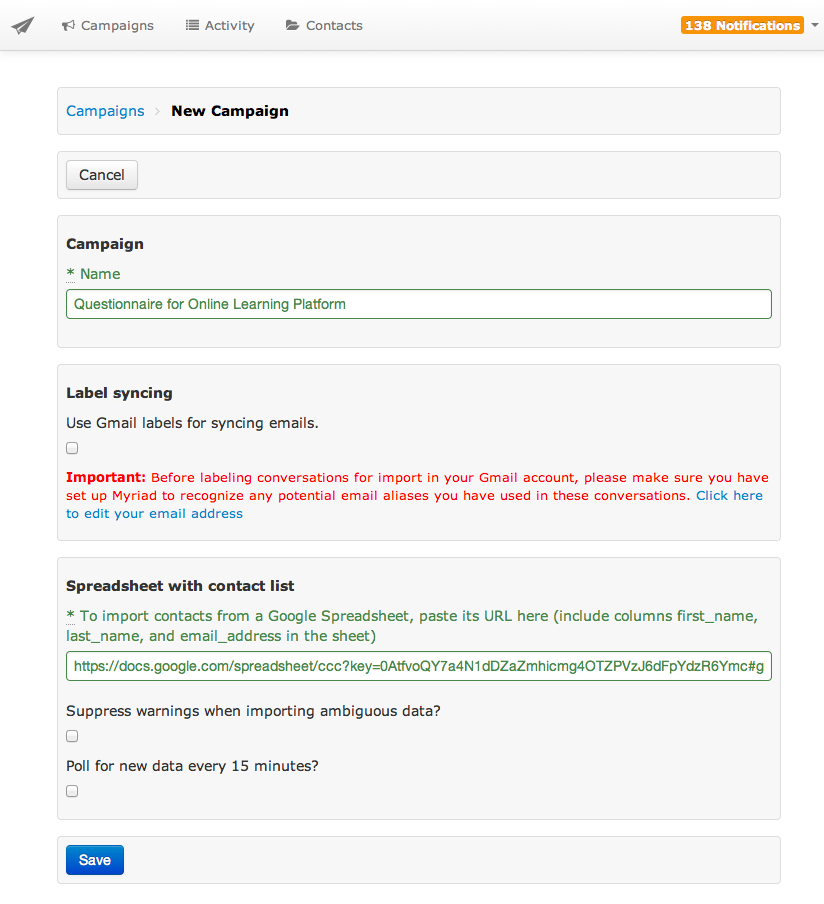
\includegraphics[width=1.00\textwidth]{imgs/CreateCampaign.png}
	\caption[Creating a Campaing in Myriad]{Creating a Campaing in Myriad}
	\label{fig:CreateCampaign}
\end{figure}

After the campaign is created, all the contacts and their \ac{KVP}s will imported if the user provided a Google Spreadsheet as in the figure \ref{fig:ContactListInCampaign}.

\begin{figure}[htbp]
	\centering
	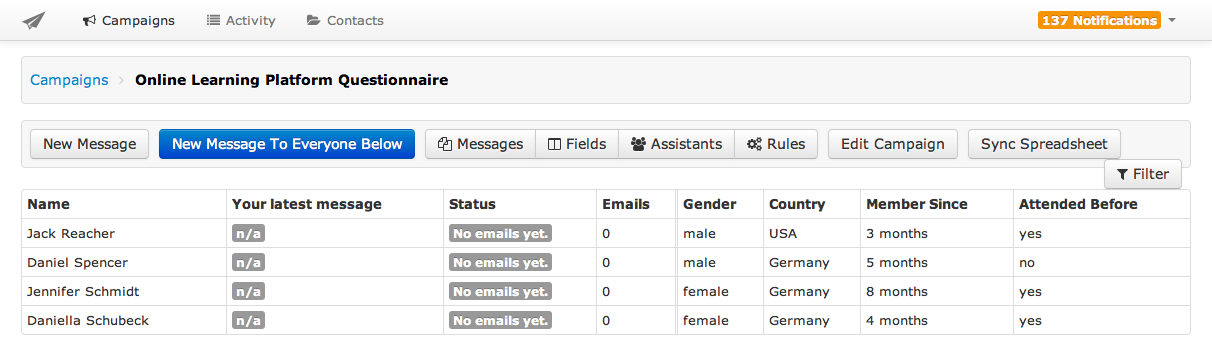
\includegraphics[width=1.00\textwidth]{imgs/ContactListInCampaign.png}
	\caption[Contacts and Their \ac{KVP}s After Synchronization in Myriad]{Contacts and Their \ac{KVP}s After Synchronization in Myriad}
	\label{fig:ContactListInCampaign}
\end{figure}

\clearpage

\subsection{Composing an Email Message}
\label{subsec:5.2.4:CompEmaiMess}

Users can send emails to all the contacts that they entered or imported into the system, or select a subset of it by using the filtering functionality as in figure \ref{fig:ContactFilters}. Provided filtering option are according to values of \ac{KVP}s, conversation status such as unread, replied, or unreplied, or the last message's template name.

\begin{figure}[htbp]
	\centering
	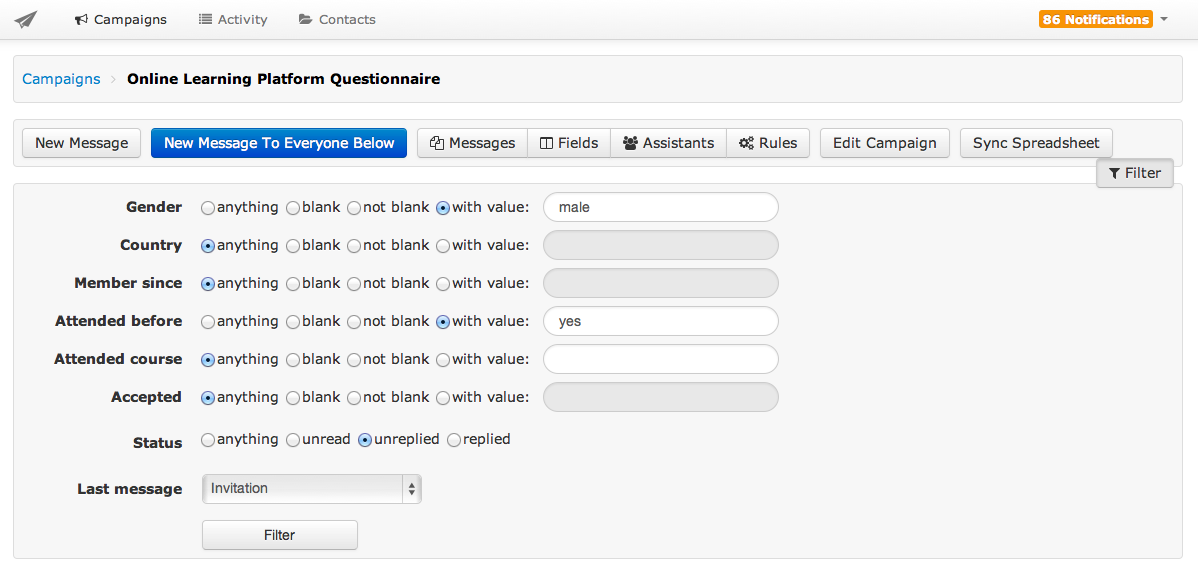
\includegraphics[width=1.00\textwidth]{imgs/ContactFilters.png}
	\caption[Filtering the Contact List in Myriad]{Filtering the Contact List in Myriad}
	\label{fig:ContactFilters}
\end{figure}

Filtered recipients are ready to be composed of email at the compose screen after pressing the corresponding button. The compose email pane (see figure \ref{fig:ComposeEmail}) contains a section that lists the previously sent emails to reuse. This is the same templating idea that was introduced at the prototype in chapter \ref{chp:4:InitIdeaProt} section \ref{subsec:4.2.2:ProtSyst}. It also shows the visualization of the state of the communication by using a tree structure, as well as the number of messages sent by using the corresponding template. A more long term campaign's visualization tree can be found in appendix \ref{app:VisuCommStat}. The system also suggest an email template while repling a responded by considering the nodes at the same tree structure.

\begin{figure}[htbp]
	\centering
	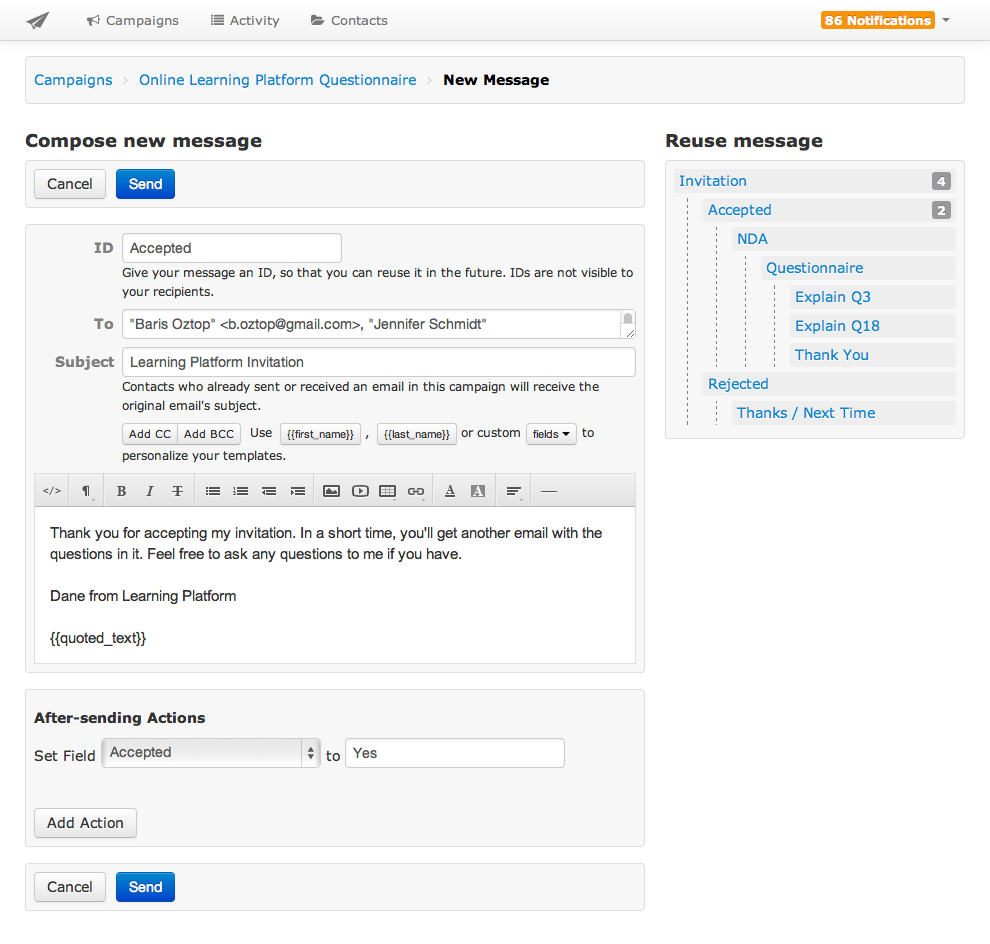
\includegraphics[width=1.00\textwidth]{imgs/ComposeEmail.png}
	\caption[Compose an Email in Myriad by Reusing Earlier Messages]{Compose an Email in Myriad by Reusing Earlier Messages}
	\label{fig:ComposeEmail}
\end{figure}

The compose pane allows users to dynamic variables into the content of messages to personalize them according to recipients. Those variables are not just limited to the first name and last name, but also can be any keys from the assigned \ac{KVP}s in the campaign.
\vspace{1cm}

\clearpage

Each campaign has a link to the other campaigns if the recipient was involved for them as well as we will see in the next section. A researcher can access to the conversations and the \ac{KVP}s from other campaigns by switching to the campaigns via that link. Providing an option to see the earlier campaigns that a recipients was involved gives broader knowledge about a recipient that may help researchers to personalize the content of the emails more easily and properly. For example, if we had extracted information regarding which sports that the recipients do in an earlier campaign. We can use the same information to make a more frankly and friendly start in the new campaign by mentioning about the latest events of those sports areas in the country. Such a technique also supports the social exchange and the diffusion of responsibility theories as discussed in section \ref{sec:2.3:PersEmai}. There is also an option to hide the \ac{KVP}s in a campaign if they are not related at all or became obsolete during the flow of the campaign to avoid cluttering of \ac{KVP}s in the application's view.
\vspace{1cm}

In the figure \ref{fig:ComposeEmail}, at the pane of "after-sending actions", users are able to set the values of the keys right after an email is sent. Therefore, a user does not need to browse another screen to change or set \ac{KVP}s whose values depends on the email user has just sent.
\vspace{1cm}

At the beginning of this section it is mentioned that a user can filter the recipients list, and send an email to the subset of it according to filtered condition. Myriad saves those filtered condition under the "Rules" menu as in the figure \ref{fig:AutomatedRules} after the user sent the email. Hence, the next time if there are new emails satisfying the same conditions as before, user will notice them under the rules menu, and the earlier sent email message can be sent to those new matching recipients automatically if user chose to enable it automated option or a user can simple press the send button manually in the same screen. For example, it the figure \ref{fig:AutomatedRules}, there are 3 recipients whose "attending" key was set to "yes", and the system already recognized that we already sent an email to those whose attending, and there are new matches for the same condition. In this case, the user can simply press the send button after, or automated the process by enabling the provided option.

\clearpage

\begin{figure}[htbp]
	\centering
	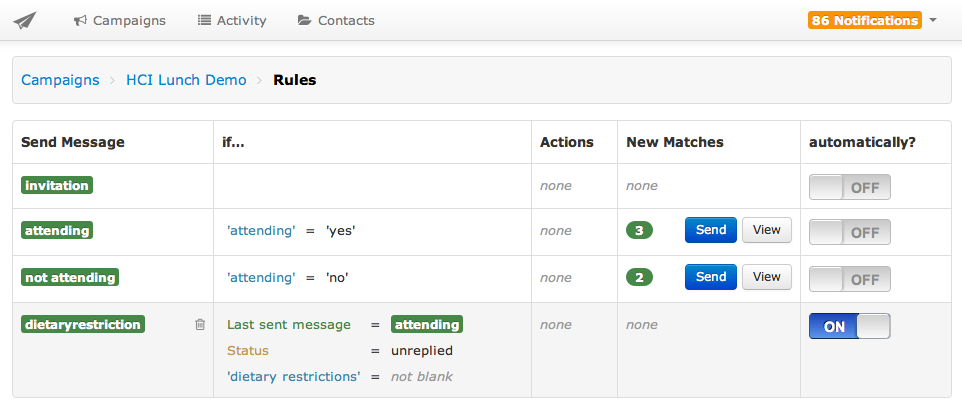
\includegraphics[width=1.00\textwidth]{imgs/AutomatedRules.png}
	\caption[Rules to Automate the Sending Process of the Emails in Myriad]{Rules to Automate the Sending Process of the Emails in Myriad}
	\label{fig:AutomatedRules}
\end{figure}

\subsection{Extracting Information from Email Messages}
\label{subsec:5.2.5:ExtrInfoEmaiMess}

Myriad's reading pane (see figure \ref{fig:MyriadReadingPane}) offers a threaded view where all the messages from a recipient are visually grouped together. The advantage of threaded view is that it allows the researcher to get a quick overview of the whole state of a conversation with an individual, therefore a researcher can write a customized message more easily by focusing on the specific personality of the individual being respond to.
\vspace{1cm}

Each of the researcher's message is also annotated with the name of the message template that was used, hence it makes the latest state of the communication easily recognizable. In the figure \ref{fig:MyriadReadingPane}, the emails that was send by the application user had a green highlighted labels writing the name of the templates that was used, which is "Accepted" and "Invitation".
\vspace{1cm}

While reading a recipient's answer, the extracted information can be recorded in \ac{KVP}s at the right-hand side of the reading pane (see figure \ref{fig:MyriadReadingPane}). Earlier recorded keys' values can be also updated at the same pane. Having \ac{KVP}s along with the conversation thread gives a researcher necessary information about the person that is going to be replied. Under the \ac{KVP} pane, a researcher can also see if the responded was involved in other campaigns with a link to those campaigns and the amount of emails that was exchanged next to it. This is an helpful feature to remind the researcher about the existing of previous relation with the respondent, and if necessary the researcher can switch to other campaign to get an overview of extracted informations in \ac{KVP}s.

\begin{figure}[htbp]
	\centering
	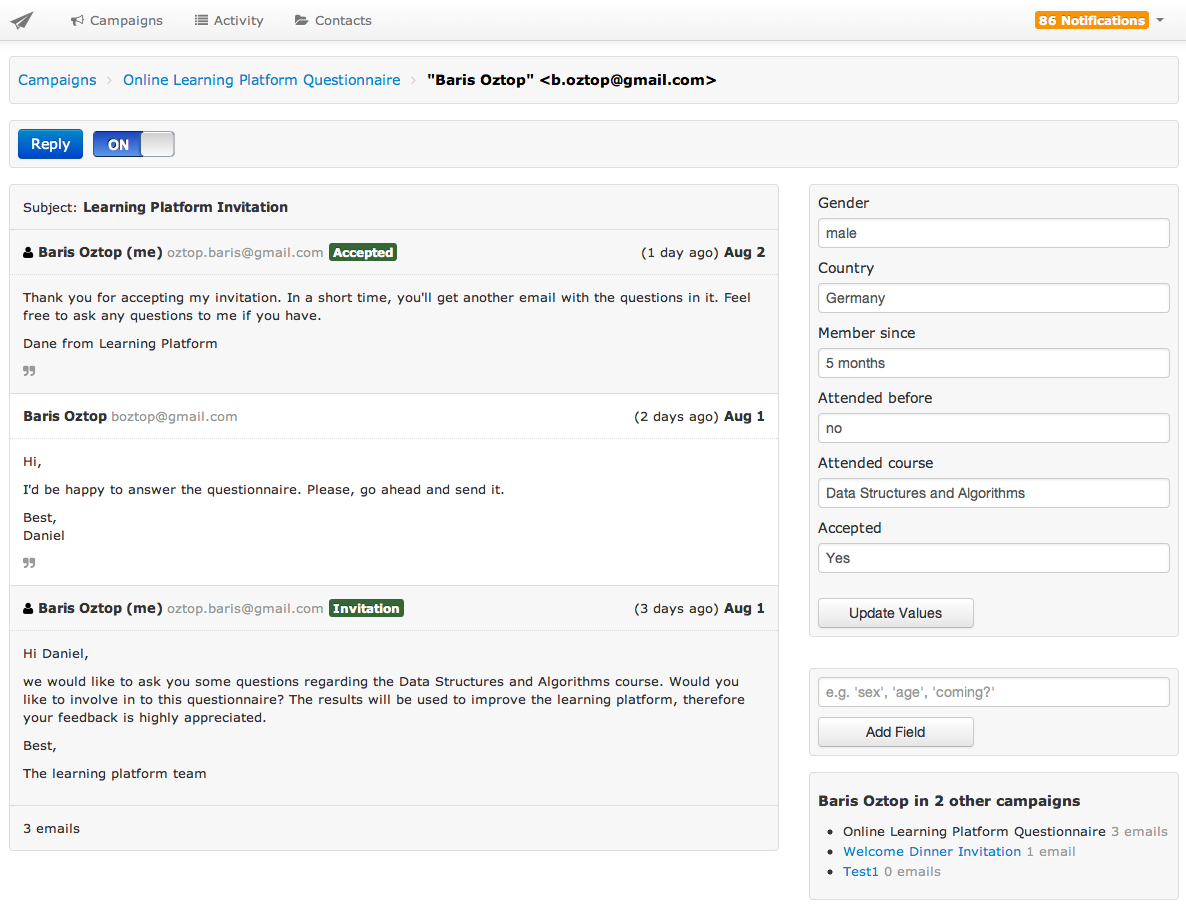
\includegraphics[width=1.00\textwidth]{imgs/MyriadReadingPane.png}
	\caption[Reading Pane and Extracted \ac{KVP}s in Myriad]{Reading Pane and Extracted \ac{KVP}s in Myriad}
	\label{fig:MyriadReadingPane}
\end{figure}

\subsection{Enabling Assistants}
\label{subsec:5.2.6:EnabAssi}

A researcher can add other researchers as assistants into a campaign by adding their Google account email addresses into Myriad as in the figure \ref{fig:AddAssistants}. The task of a researcher can be extracting information from the email, writing answer to the recipients, or even proofreading of a researcher's emails before sending them.

\clearpage

\begin{figure}[htbp]
	\centering
	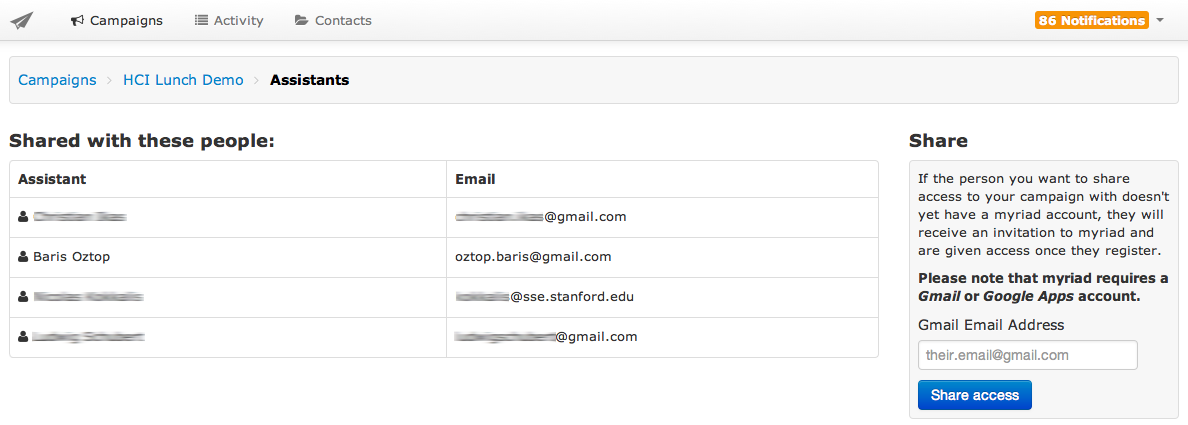
\includegraphics[width=1.00\textwidth]{imgs/AddAssistants.png}
	\caption[Rules to Automate the Sending Process of the Emails in Myriad]{Rules to Automate the Sending Process of the Emails in Myriad}
	\label{fig:AddAssistants}
\end{figure}

After an assistant is assigned to a campaign, he or she will get an notification email including the link to the campaign. Again, there will be a notification email for each email coming from respondents to the assistants' email address to let them know about the action required situation.
\vspace{1cm}

Myriad provides status labels for each received or sent email to give a hint about the next required actions as in the figure \ref{fig:EmailStatuses}. These status labels give a hint about the next action that should be done in the state the conversation such as if the application user needs to read or reply a message, or the action is required from the recipient's side to continue the communication. There are also status labels related with Myriad's internal state regarding to an email message such as if Myriad sent the messages, or there was a failure with sending. The same view also provides a column to show what was the last message that is sent by an application user. Therefore, researchers and assistants will easily realize what should be done next, and see the status of the communication for each recipient. 

\clearpage

\begin{figure}[htbp]
	\centering
	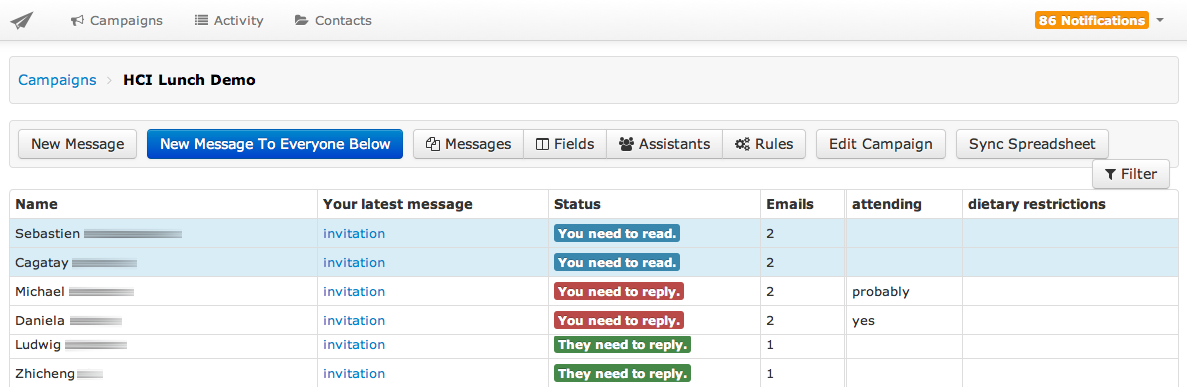
\includegraphics[width=1.00\textwidth]{imgs/EmailStatuses.png}
	\caption[Status Labels for Each Email in Myriad]{Status Labels for Each Email in Myriad}
	\label{fig:EmailStatuses}
\end{figure}

\section{Architecture}
\label{sec:5.3:FinaArch}

As it was at the prototype, Myriad was also developed using framework stack of \ac{RoR}, jQuery, Bootstrap, and OAuth\footnote{OAuth is leveraged by using OmniAuth library (https://github.com/intridea/omniauth), and its Google authentication strategy is implementation by OmniAuth Google OAuth2. Details can be found at https://github.com/zquestz/omniauth-google-oauth2} protocol was used for authentication with Gmail. Initial project structure was generated by a gem named Rails Apps Composer\footnote{https://github.com/RailsApps/rails\_apps\_composer}, which consists a collection of Rails application templates to start a project. Thanks to the other gems that we used along the way of the development to make this project completed on time in a robust way. In the next sections, we will see the implementation details of Myriad, and how it makes a mass email communication possible.

\subsection{Keeping Track of Recipients}
\label{subsec:5.3.1:ReciCont}

It was mentioned in section \ref{sec:4.2:Prot}, the prototype didn't keep information regarding to the recipients, but about the messages that they sent. Therefore, the extracted information, which are \ac{KVP}s, was related to the email messages of the recipients. The side effect of this approach was not the able get all the \ac{KVP}s of the recipients at one glance instead browsing by the earlier emails of the recipients, and each time we had to create the same key for each recipients since the system was not aware if it was already created for other email in the same campaign.
\vspace{1cm}

In Myriad, we overcame this issue by keeping all the recipients information in a separate data model named contact as in the figure \ref{fig:UML_Draw_Final}. Hence, we are able to keep track of recipients among different campaigns via the conversations of them, which is another data model in the Myriad as each campaign has many conversations of a recipient.
\vspace{1cm}

Myriad keeps the basic profile information of the recipients which are the first names, last names, and email addresses. Those information can be imported into Myriad by the spreadsheet synchronization, by adding them into "To" filed when user compose an email, or by importing from Gmail's inbox via the label synchronization. The recipients' email addresses are unique identifier for Myriad to compare already existing recipient information with the synchronized ones. 

\begin{figure}[htbp]
	\centering
	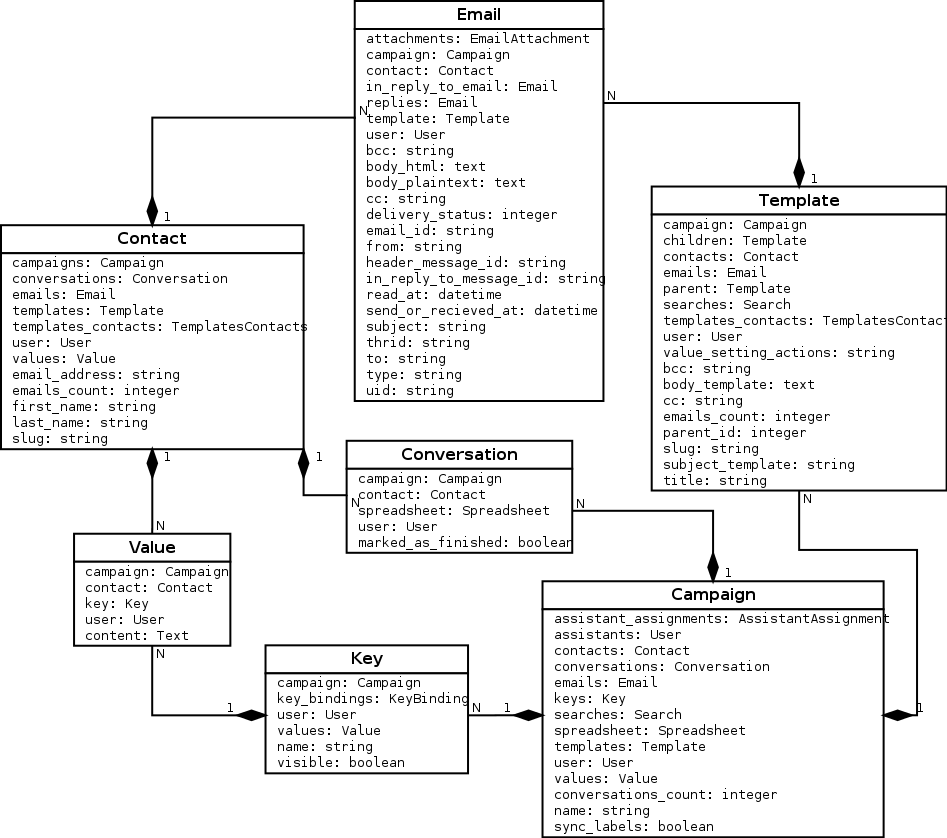
\includegraphics[width=1.00\textwidth]{imgs/UML_Draw_Final.png}
	\caption[Model Dependency of the Myriad Compared with the Prototype]{Model Dependency of the Myriad Compared with the Prototype}
	\label{fig:UML_Draw_Final}
\end{figure}

\subsection{The \ac{KVP}s and the Templates}
\label{subsec:5.3.2:KVPsTemp}

Having a separate contact data model to keep track of recipients also made us to relate each extracted information, namely \ac{KVP}s, to them, instead of their message in a campaign as in figure \ref{fig:UML_Draw_Final}. Each campaign has many keys, and their values are according to recipients. One advantages of this is when we browse to a conversation of a recipient, we are able to see all the \ac{KVP}s of that recipients under one view, which was the \ac{KVP} pane next to the email threads in the figure \ref{fig:ComposeEmail}. The other benefit comes at the synchronization with spreadsheet. When a new key is added to a recipient or a value of a key is updated via Myriad, it will be reflected to the spreadsheet as well. Therefore, the spreadsheet will always contain the latest changes done by user in Myriad. 
\vspace{1cm}

As it was in the prototype, the templates contains emails messages with dynamic variables in it, and the actual emails whose dynamic variables are filled with values are kept in the Email data model as in the figure \ref{fig:UML_Draw_Final} after they are fetched from Gmail.
\vspace{1cm}

To visualize the state of the conversation, and let the users select templates, Myriad offers the tree structure as it was in the prototype. However, the implementation of the tree structure is different from the prototype. In section \ref{subsec:4.2.3:ProtArch}, it was mentioned that the hierarchy between the nodes of the tree was a nested set model. We decided to use adjacency list model instead of nested set model to increase the readability of the templates' relation at the data model level from the developers' perspective. Since the relation of the templates is not as completed as in other relations, the performance drawbacks on this decision was negligible. 

\subsection{A Campaign Message Identification}
\label{subsec:5.3.3:MessIden}
At the prototype, due to dependency on the existing EmailValet's email fetching process, we were identifying the emails which belongs to a campaign, then inserting them into the same inbox in EmailValet. With Myriad, we removed this dependency, and only consider and show the emails which belongs to a campaign.
\vspace{1cm}

The identification of the emails depends on the three different conditions:

\begin{compactenum}
	\item The emails that are fetched from Gmail and reply to one of to the campaign message.
	\item The emails that are composed in Myriad as a part of the campaign whether they are the emails to initiate a campaign or replies to the recipients' emails.
	\item The emails that are imported into Myriad from Gmail's inbox via label synchronization (see section \ref{} for label synchronization)
\end{compactenum}

Myriad initially retrieves all the email's \ac{UID}s\footnote{UID (Unique Identifier) is 32-bit integer value to uniquely identify emails in a mailbox in \ac{IMAP}. Each email added into mailbox will have a higher value than the ones added before, however they are not necessarily contiguous \citep{rfc3501}. \ac{UID} is used as it was in the prototype by the implementation of the EmailValet's part. It is used to identify if a message is already fetched from Gmail, if it is not, it is fetched since it is a new message.} from Gmail's inbox of the last 14 days instead of all the emails of the inbox to reduce the time consumption of the fetching process. For those \ac{UID}s whose not stored in Email data model in Myriad, Myriad retrieves the actual email along with the metadata such as Gmail thread ID\footnote{Gmail thread ID is a 64-bit integer that is part of the provided Gmail's IMAP extension. It helps to associate groups of messages in the same manner as in the Gmail web interface \citep{GoogleInc.2013a}.} and Gmail labels.
\vspace{1cm}

As it was in the prototype, we set a message-ID to the emails that are composed in Myriad. Therefore, we are able to identify during the aforementioned fetching process whether an email from Gmail is the one that was composed to initiate a campaign or was a reply to the one of the recipients email in a campaign by a Myriad user. Message-ID field is again leveraged for identifying the recipients messages belonging to a campaign. Myriad retrieves the Message-ID written in the In-Reply-To, and checks if it matches one of the campaign messages in Myriad. Another field that Myriad checks is the "References" field\footnote{Reference field in another identification field along with Message-ID defined by RFC 5322. It contains one or more Message-IDs used when creating a reply to a message to identify the original message or the other messages when a reply to a message that was itself a reply \citep{rfc5322}.} to identify the messages belongs to a campaign but forwarded to another person by the recipients in order to reply the message. Since the forwarded endpoint's email client sets the Message-ID of the forwarded message into the In-Reply-To, which is not known at all by Myriad, Myriad checks the "References" field to identify a Message-ID that belongs to a campaign in this case. This scenario is illustrated in the figure \ref{fig:drawingMessageReferences}.

\begin{figure}[htbp]
	\centering
	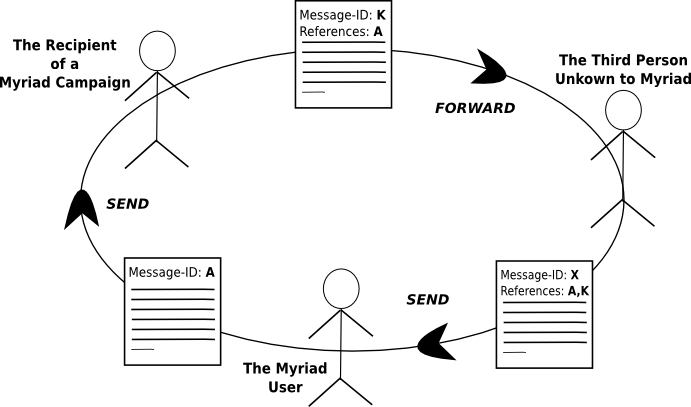
\includegraphics[width=1.00\textwidth]{imgs/drawingMessageReferences.png}
	\caption[A Scenario Using References Field in an Email]{A Scenario Using References Field in an Email}
	\label{fig:drawingMessageReferences}
\end{figure}

If an email is not identified as a campaign message by comparing the Message-IDs with the ones in Myriad's Email data model, the next step is to evaluate those emails in case of they were labelled as a Myriad campaign in the Gmail's inbox. In this case, if an email has a label in the pattern of "myriad/campaign-name", and there is already a created campaign in Myriad with the name "Campaign Name", that email will be stored in the data model. Finally, an identified email will be assigned to a contact by looking its parent email's Message-ID if it was a reply or if it fails the contact information will be recorded from the email's "From" header field. The rest of the emails will be ignored since there were no matches found in the mentioned email header fields, which are Message-ID, In-Reply-To, and References, or Gmail's Label.

\section{Experiences}
\label{sec:5.5:Expr}

\section{Conclusion}
\label{sec:5.4:Conc}

\begin{comment}

--> Gmail labellari ni anlatirken, diger urunlerde import nasil email forwardingle yapiliyordu onu anlat kesin.


However, we still needs to supply a system, where it offers a work flow to make it happen. satisfy these 

distribution of the work

initial idea is reducing effort as we disscussed


Requirements'dan once urunu tanit screenshot'larla cunku cok zaman kaybedecen


write first about the revised requirements,
then describe the product with pictures,
then some technical details

\section{Product}
\label{sec:5.1:FinaProd}

\subsection{Improved Requirements}
\label{subsec:5.1.1:Cust}

\subsection{Final System}
\label{subsec:5.1.2:FinaSyst}

\subsection{Architecture}
\label{subsec:5.1.3:FinaArch}

-------------
chapter 6
-------------
Evaluation
- Experiences
- Statistics
- Conclusion

\end{comment}
